\documentclass[tikz,border=5pt]{standalone}
\usepackage{tikz}
\usetikzlibrary{shapes,backgrounds}
\begin{document}
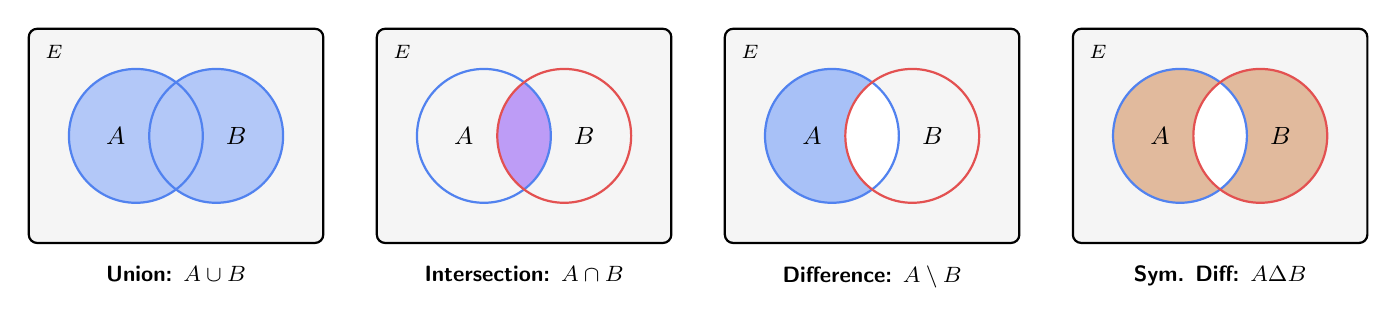
\begin{tikzpicture}[scale=0.85]
  \definecolor{setblue}{HTML}{2563EB}
  \definecolor{setred}{HTML}{DC2626}
  \definecolor{setpurple}{HTML}{7C3AED}
  \definecolor{ambergold}{HTML}{B45309}

  % Subfigure 1: Union
  \begin{scope}[shift={(0,0)}]
    \draw[thick, rounded corners=3pt, fill=gray!8] (-2.2,-1.6) rectangle (2.2,1.6);
    \node[anchor=north west, font=\sffamily\scriptsize\bfseries] at (-2.1,1.5) {$E$};
    \fill[setblue!35] (-0.6,0) circle (1.0);
    \fill[setblue!35] (0.6,0) circle (1.0);
    \draw[thick, setblue!80] (-0.6,0) circle (1.0);
    \draw[thick, setblue!80] (0.6,0) circle (1.0);
    \node[font=\sffamily\small\bfseries] at (-0.9,0) {$A$};
    \node[font=\sffamily\small\bfseries] at (0.9,0) {$B$};
    \node[below, font=\sffamily\footnotesize\bfseries] at (0,-1.8) {Union: $A \cup B$};
  \end{scope}

  % Subfigure 2: Intersection
  \begin{scope}[shift={(5.2,0)}]
    \draw[thick, rounded corners=3pt, fill=gray!8] (-2.2,-1.6) rectangle (2.2,1.6);
    \node[anchor=north west, font=\sffamily\scriptsize\bfseries] at (-2.1,1.5) {$E$};
    \begin{scope}
      \clip (-0.6,0) circle (1.0);
      \fill[setpurple!50] (0.6,0) circle (1.0);
    \end{scope}
    \draw[thick, setblue!80] (-0.6,0) circle (1.0);
    \draw[thick, setred!80] (0.6,0) circle (1.0);
    \node[font=\sffamily\small\bfseries] at (-0.9,0) {$A$};
    \node[font=\sffamily\small\bfseries] at (0.9,0) {$B$};
    \node[below, font=\sffamily\footnotesize\bfseries] at (0,-1.8) {Intersection: $A \cap B$};
  \end{scope}

  % Subfigure 3: Difference
  \begin{scope}[shift={(10.4,0)}]
    \draw[thick, rounded corners=3pt, fill=gray!8] (-2.2,-1.6) rectangle (2.2,1.6);
    \node[anchor=north west, font=\sffamily\scriptsize\bfseries] at (-2.1,1.5) {$E$};
    \begin{scope}
      \fill[setblue!40] (-0.6,0) circle (1.0);
      \clip (0.6,0) circle (1.0);
      \fill[white] (-0.6,0) circle (1.0);
    \end{scope}
    \draw[thick, setblue!80] (-0.6,0) circle (1.0);
    \draw[thick, setred!80] (0.6,0) circle (1.0);
    \node[font=\sffamily\small\bfseries] at (-0.9,0) {$A$};
    \node[font=\sffamily\small\bfseries] at (0.9,0) {$B$};
    \node[below, font=\sffamily\footnotesize\bfseries] at (0,-1.8) {Difference: $A \setminus B$};
  \end{scope}

  % Subfigure 4: Symmetric Difference
  \begin{scope}[shift={(15.6,0)}]
    \draw[thick, rounded corners=3pt, fill=gray!8] (-2.2,-1.6) rectangle (2.2,1.6);
    \node[anchor=north west, font=\sffamily\scriptsize\bfseries] at (-2.1,1.5) {$E$};
    \fill[ambergold!40] (-0.6,0) circle (1.0);
    \fill[ambergold!40] (0.6,0) circle (1.0);
    \begin{scope}
      \clip (-0.6,0) circle (1.0);
      \fill[white] (0.6,0) circle (1.0);
    \end{scope}
    \draw[thick, setblue!80] (-0.6,0) circle (1.0);
    \draw[thick, setred!80] (0.6,0) circle (1.0);
    \node[font=\sffamily\small\bfseries] at (-0.9,0) {$A$};
    \node[font=\sffamily\small\bfseries] at (0.9,0) {$B$};
    \node[below, font=\sffamily\footnotesize\bfseries] at (0,-1.8) {Sym. Diff: $A \Delta B$};
  \end{scope}
\end{tikzpicture}
\end{document}